\section{Testy a continuous integration}
W celu lepszego zrozumienia istoty automatyzacji testów konieczne jest najpiew zrozumienie testów samych w sobie. Jak zostało to opisane w rozdziale 1.4 - pisanie testów jest integralną częścią pracy każdego programisty. Wiele osób uważało to dawniej za żmudne zadanie, nieprzynoszące wymiernych korzyści, jednakże z biegiem czasu stało się jasne, że w dużych projektach informatycznych są one konieczne, co widać w dzisiejszych czasach w wypowiedziach wielu osób. \cite{UnitOpinions} \cite{UnitResults}
\begin{figure}[htbp]
    \centering
    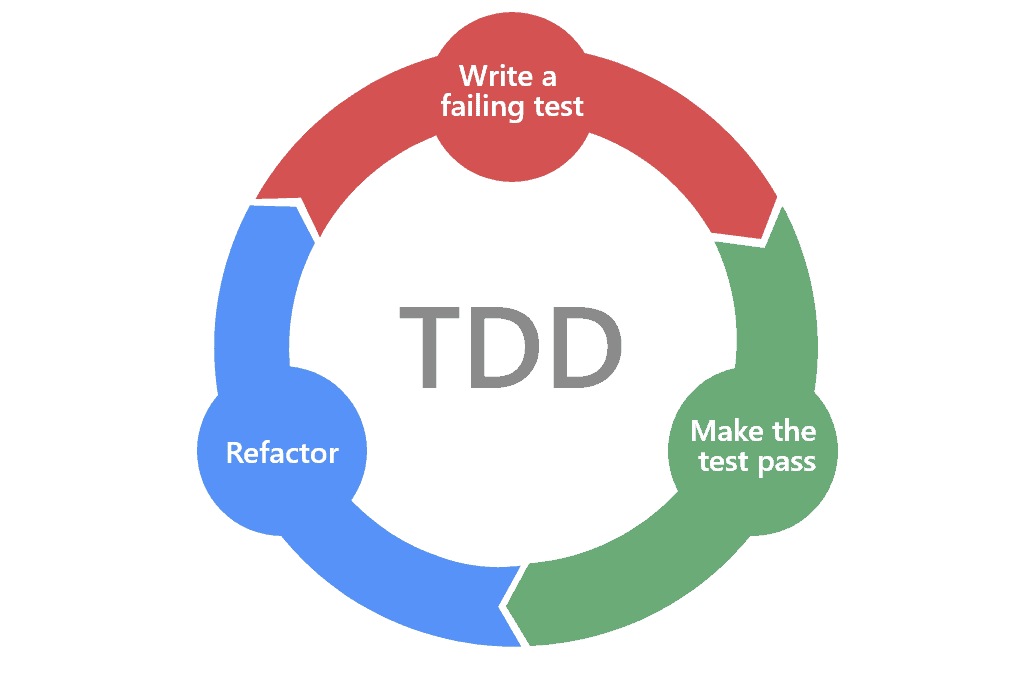
\includegraphics[width=10cm]{images/tdd.png}
    \caption{Zasada Red-Green-Refactor}
    \label{fig:redgreen}
\end{figure}
\par Najpopularniejsze obecnie są dwie metody pisania testów: 
\begin{itemize}
    \item TDD - Test Driven Development - zaproponowana została przez Kenta Becka w 2002 roku. \cite{TestDrivenDevelopment} Zakłada, że testy będą napędzały tworzenie projektu i stały u jego podstawy. 
    \par Pierwszym krokiem przy implementacji nowej funkcji w naszym projekcie powinno być napisanie samego testu, który oczywiście na początku nie powiedzie się, ponieważ kod, który ma on testować nie został jeszcze napisany. Po napisaniu testu przechodzi się do pisania kodu, który w jak najłatwiejszy sposób będzie w stanie zaliczyć napisany przez nas test. Ostatnim krokiem tego cyklu jest refactoring kodu, polepszający jego jakość, tak aby spałniał on oczekiwane standardy.
    Takie podejście pozwala na tworzenie dobrze zaprojektowanego kodu, który jest w całości pokryty testami, co owocuje w przyszłości, kiedy konieczne jest wprowadzanie zmian w bazie kodu.
    
    \item BDD - Behavior Driven Development - metodologia zaproponowana przez Dana Northa w 2006 roku. Zakłada ona zaangażowanie w tworzenie oprogramowania osób nietechnicznych - analityków oraz klientów dla których oprogramowanie jest tworzone. Testy tworzone są według zasady "Given - When - Then (Zakładając - Gdy - Wtedy)". Można w ten sposób łatwo opisać testy, które każdy będzie w stanie zrozumieć, a następnie zaimplementować przy użyciu odpowiedniego frameworka, np. JBehave dla Java lub Behave dla Pythona. 
\end{itemize}

\begin{figure}[htbp]
    \centering
    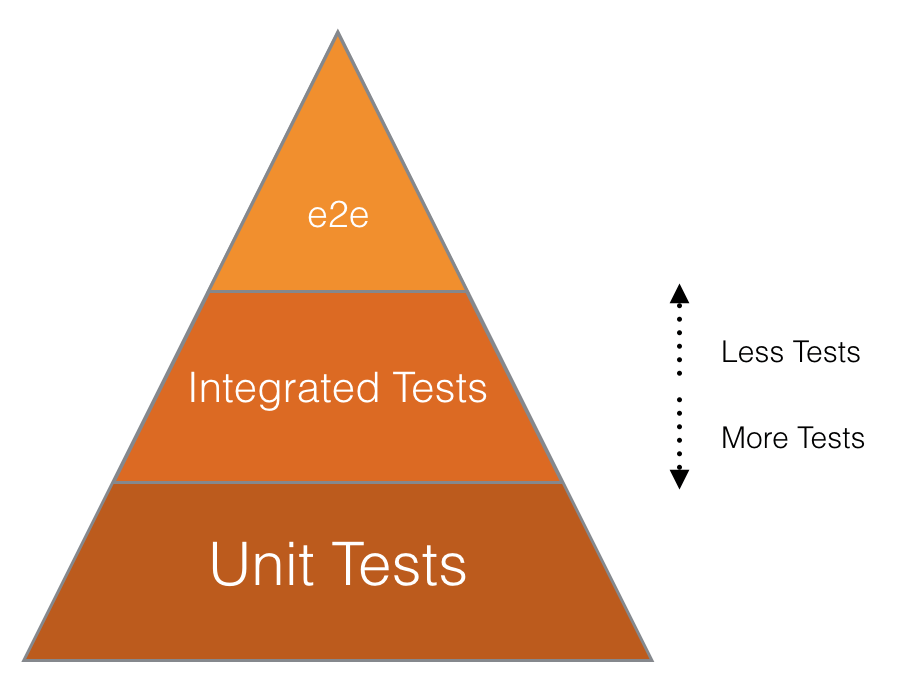
\includegraphics[width=10cm]{images/testing_triangle.png}
    \caption{Piramida testów}
    \label{fig:testing}
\end{figure}



\subsection{Testy jednostkowe}
Testem jednostkowym nazywa się kod, który jest w stanie wywołać inny fragment kodu programu, a nastepnie sprawdzić czy działanie tamtego kodu jest zgodne z zakładanym przez programistę działaniem. \cite{UnitDefinition}
\par Autor tej definicji zdefiniował też kilka warunków, które powinien spełniać każdy test jednostkowy: 
\begin{itemize}
    \item jest w pełni zautomatyzowany
    \item może być wykorzystywany w wielu miejscach, także jako część innych testów
    \item działa w pamięci, bez dostępu do baz danych lub plików
    \item jest deterministyczny, nie zawiera losowych danych
    \item jest szybki
    \item skupia się na pojedynczym logicznym elemencie programu
    \item czytelny
    \item łatwy w zrozumieniu
    \item wiarygodny 
\end{itemize}
Fragmentem kodu, który podlega testom jest zwykle najmniejszy jego fragment, który odpowiada za jedno logiczne działanie. Najczęściej będzie to pojedyczna metoda klasy, cała klasa lub rzadziej nawet kilka klas. Odpowiednie przygotowanie testów jest kluczowe jeśli chcemy uniknąć w naszym projekcie regresji - pojawienia się błędów w kodzie, który wcześniej działał poprawnie. 

\begin{lstlisting}[caption={Test jednostkowy w języku Python}]
    
    TODO przykladowy kod
\end{lstlisting}
\subsection{Testy integracyjne}

\subsection{Testy end-to-end}

\subsection{Rola CI w testach}

\subsection{Przykład w GitHub Actions}